Elosztott rendszer Erlang-ban lett megvalósítva. Az elosztást interpolációnként végezzük, vagyis annyi processzt hozunk létre amennyi interpolációt kívánunk egyszerre kiszámítani. \newline
A szerver figyel egy portot hogy érkezett-e rá adat. Ha érkezett adat az adott portra, azt kibontja, és elvégzi a szükséges műveleteket. Kinyer belőle egy listát mely az interpolálni kívánt pontokat és tulajdonságokat tartalmazza. \newline
Tudjuk pontosan hány eleme van a listának, és annyi processzt hozunk létre. Ha vannak felcsatlakozva node-ok akkor a processzt az adott node-on is meg tudja hívni.
Ha létrehozta a processzeket lista elemein végig megy, és azokat szétküldi a processzeknek, majd megvárja míg az összes végig ér, és visszatérve megkapja az eredményt.
\subsection{Web-szerver kommunikáció}
	A webszerver kommunikációhoz a fájlok a httpServer.erl fájlban találhatóak meg. Az ebben található függvényeket a main-ben hívjuk meg amikor inicializáljuk a szervert.

	%%\ref{fig:call_graph_serverconfig}
	\begin{figure}[h]
		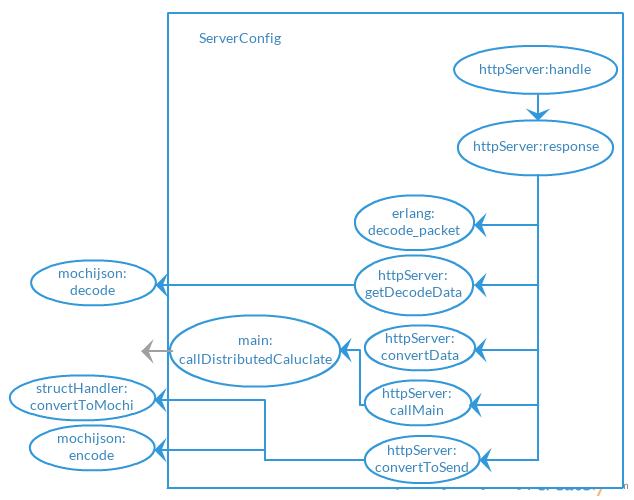
\includegraphics[width=13cm]{pics/call_graph_serverconfig}
		\centering
		\caption{Szerver hívási folyamata\label{fig:call_graph_serverconfig}}
	\end{figure}

	\begin{description}
	\item[httpServer:start(Port, WatcherNode)] 
		\hfill \\
		Elindítja a szervert, az adott porton. \newline
		Ezt a függvényt a main-ben hívjuk, meg ahol már megkapja a node-figyelő pid-jét és az alapértelmezett port-ot.
	\item[httpServer:response(Str, WatcherNode)] \hfill \\ 
		Miután érkezik egy kérés a szervernek ebben a függvényben kezeljük le. Innen indul ki minden folyamat ami a számítást végzi. \newline 
		Az alábbi sorrendben hívódnak meg a függvények: \newline
		getDecodeData, convertData, callMain, convertToSend.
	\item[httpServer:getDecodeData(\_)] \hfill \\ 
		Visszatér a szervernek küldött paraméterrel.
	\item[httpServer:convertData(ResponseParams)] \hfill \\ 
		Létrehozza a kapott adatból az Erlang struktúrát.
	\item[httpServer:callMain(RespJson, WatcherNode)] \hfill \\ 
		Amikor az adatokat feldolgoztuk és minden rendben ment, elindítjuk a main függvényét, ezen függvény segítségével.
	\item[httpServer:convertToSend(Object)] \hfill \\ 
		Amikor a számítás véget ért, létrehozzunk a visszaküldéshez szükséges adatstruktúrát, majd elküldjük a szervernek.
	\end{description}
\subsection{Adat feldolgozás}
	Az adatot JSON-ben kapja a szerver. Az adathalmaz kibontásához MonchiJSON lett alkalmazva. 
	A segédfüggvények és konvertálók a \texttt{Utility/structHandler.erl} fájlban lettek megvalósítva.\newline
	Elsősorban a megkapott speciális adathalmaz kibontására használtak az itt lévő függvények, de egyéb segédfüggvények is megtalálhatóak ebben a fájlban, amelyek a konvertálással kapcsolatosak.

	\subsubsection{\underline{
		Mochi-json kibontásához használt segédfüggvények:
	}}
	\begin{description}
		\item[structHandler:getElementByKeyList(KeyList, DataSetElement)] \hfill \\ 
		Visszatér egy értékkel, amely az adott kulcson van, ha egy elemű a kulcs lista. Több elem esetén a kulcsokban lévő értékeket nézi, és visszaadja a legbelső kulcson lévő elemet.

		\item[structHandler:getElementByKey()] \hfill \\ 
		Visszatér egy objektumban az adott kulcson lévő értékkel.
	\end{description}
	A struktúra-kezelő interpoláció meghívásához használt függvényei:
	\begin{description}

		\item[structHandler:getDataByJson(JsonSting)] \hfill \\
		A mochi-json dekódoló meghívása, visszatér egy Erlang struktúrával.
		
		\item[structHandler:getDataSet(Data)]\hfill \\ 
		Visszatér az adatok halmazával. Ebből a halmazon, vagyis listán kell végig menni, és szétosztani az elemeit. 
		
		\item[structHandler:getPoints] \hfill \\
		Pontok visszanyerése egy speciális módon, melyet a \texttt{calulator} fel tud használni.

				\begin{minted}{erlang}
EmptyStruct =  [{x, []}, {y, []}]
		\end{minted}


		\item[structHandler:<Számítási paraméterek>] \hfill \\ 
		getInverse(DataSetElement) - inverz-e \newline
		getType(DataSetElement) mi a típusa? \newline
		getId(DataSetElement) egyedi azonosítója \newline
		getPoints(DataSetElement) pontok struktúrája
	\end{description}
	Az eredmény visszanyeréséhez az alábbi segédfüggvényeket kellett használni:
	\begin{description}
	
		\item[structHandler:convertToMochi(Object)] \hfill \\ 
		A mochi-json Erlang struktúra annyira nem egyértelmű elemekből áll. Speciálisan kell felépíteni az eredményt. Ez a függvény megkap egy Erlang listát és átkonvertálja mochi-json-nak megfelelő struktúrává, majd átkonvertálja egy json string-gé.

		\item[structHandler:simplifyPolinomial(Result, Array) ] \hfill \\ 
		Egyszerűsíti a polinomot amelyet eredményül kapott.
	
	\end{description}
\subsection{Gép-szerver kommunikáció}
	\begin{description}
	\item[pidWatch:startPidWatch()]
	\hfill \\ Elindítja a node-figyelőt, melyben feliratkozni lehet a listára, vagy lekérdezni az adatokat. A node-figyelő indulás után figyelni fog és ha küldenek neki egy kérést, akkor azt kezeli. 
	\item[pidWatch:registerToServer(Pong\_Node)]
	\hfill \\ Ezzel a kéréssel lehet felcsatlakozni a szerverre. A kérést elküldi és ha sikeres volt a feliratkozás, akkor ok-al tér vissza.
	\end{description}
\subsection{Elosztás megvalósítása}
	Az elosztást tartalmazó fájlokat a /DistributedSystem mappában találjuk meg. nodeHandler.erl fájlban találhatóak a processz létrehozással kapcsolatos függvények. fork.erl fájlban a processz kommunikáció logikája van megvalósítva.

	%%\ref{fig:call_graph_distributed1}
	\begin{figure}[h]
		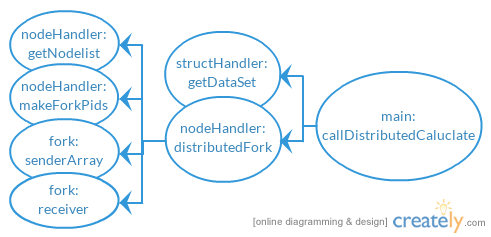
\includegraphics[width=10cm]{pics/call_graph_distributed1}
		\centering
		\caption{Elosztás folyamat hívásai\label{fig:call_graph_distributed1}}
	\end{figure}

	%%\ref{fig:call_graph_distributed1}
	\begin{figure}[h]
		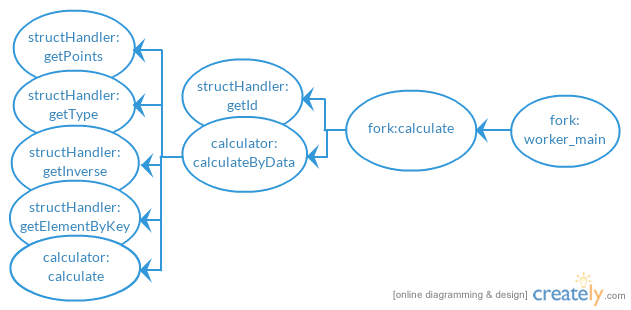
\includegraphics[width=12cm]{pics/call_graph_distributed2}
		\centering
		\caption{Gyerek folyamat hívásai\label{fig:call_graph_distributed2}}
	\end{figure}
	
	\begin{description}
		\item[nodeHandler:distributedFork(NumOfPids, DataList, WatcherNode)]
		\hfill \\
		Létrehozza a számításhoz szükséges node Struktúrát.
		LogicModule-ban szereplő senderstart, recivestart, worker\_main függvényeket kezeli.
		\item[nodeHandler:getNodelist]
		\hfill \\
		Lekéri a node-figyelőtől a felcsatlakozott node-okat.
		\item[nodeHandler:makeForkPids]
		\hfill \\
		Létrehozza a számításhoz szükséges új processzeket.

		\item[fork:senderArray]
		\hfill \\ 
			Végig megy egy adott tömbön és az elemeit szétküldi a processzeknek. 
		\item[fork:receiver]
		\hfill \\
			Válaszok érkezésére vár a processzektől. Ha minden válasz megérkezett, akkor visszatér.
		\item[fork:worker\_main]
		\hfill \\
			A gyerek processzek függvénye. Várja a szülőtől az adatot, számol vele és visszaküldi.
		\item[fork:calculate]
		\hfill \\ 
			A fork-ból a számítást hívó függvény. Eredménnyel visszatér, majd azt olyan formára hozza, amit vár a szülő. 
	\end{description}